\documentclass[12pt,letterpaper]{article}
\usepackage[left=.91in,right=.91in,top=.77in,bottom=.76in,footskip=.36in]{geometry}
\usepackage{amsmath,array,tabularx,booktabs,tikz,hyperref}
\hypersetup{hidelinks,pdftitle={Ask the Notes: A practical guide},pdfauthor={Juan Salinas}}
\ifdefined\XeTeXversion
  \IfFileExists{/System/Library/Fonts/Monaco.ttf}{
    \DeclareFontFamily{TU}{guidemono}{}
    \DeclareFontShape{TU}{guidemono}{m}{n}{<-> "[/System/Library/Fonts/Monaco.ttf]"}{}
    \renewcommand{\ttdefault}{guidemono}
  }{}
\fi
\raggedright\setlength{\parindent}{0pt}\setlength{\parskip}{5pt}
\setlength{\emergencystretch}{1.6em}
\newcommand{\topline}[1]{{\small MATH 1334\quad / \quad Ask the Notes\hfill #1\par}\vspace{5pt}\hrule\vspace{11pt}}
\newcommand{\titleline}[1]{{\huge\bfseries #1\par}\vspace{2pt}}
\newcommand{\hd}[1]{\par\addvspace{9pt}{\large\bfseries #1\par}\nobreak}
\newcommand{\step}[2]{\par\addvspace{5pt}\textbf{#1.\enspace #2}\par\nobreak}
\newcommand{\file}[1]{{\small\texttt{\detokenize{#1}}}}
\newcommand{\lnk}[2]{\href{#1}{\underline{#2}}}
\newcommand{\jump}[2]{\hyperlink{#1}{\underline{#2}}}
\newcommand{\partpage}[3]{\newpage\hypertarget{#1}{}\pdfbookmark[0]{#3}{mark-#1}\topline{#2}\titleline{#3}}
\newcolumntype{Y}{>{\raggedright\arraybackslash}X}
\newcommand{\grid}[2]{\par\smallskip{\renewcommand{\arraystretch}{1.23}\begin{tabularx}{\linewidth}{@{}>{\raggedright\arraybackslash}p{#1}@{\hspace{13pt}}Y@{}}\toprule #2\bottomrule\end{tabularx}}\par}
\newcommand{\repo}{https://github.com/juansalinas2/Math-1334---Calculus}
\newcommand{\book}{https://juansalinas2.github.io/Math-1334---Calculus}
\begin{document}
\pdfbookmark[0]{Try Ask}{mark-start}
\topline{Instructor's practical guide \quad / \quad November 2026}
\titleline{Ask the Notes}
{\large How the calculus tutor finds a problem, teaches a step, and cites your notes.\par}
\hd{Try one conversation}
Open \lnk{\book/lectures/exam-3-review.html\#products-and-powers}{Exam 3 review, problem 12}. Part (c) asks for \(\lim_{x\to\infty}x^{1/x}\). Open \textbf{Ask}, enter the class code if prompted, and try these two turns. Compare the mathematics and the source link. The tutor's wording can vary.
\grid{.29\linewidth}{
\textbf{What you type}&\textbf{What a useful reply does}\\\midrule
\emph{Just a hint for 12(c).}&Sets \(y=x^{1/x}\) and suggests taking \(\ln y\). Leaves you to form the quotient.\\
\emph{I got zero for the logarithm. Does that make the original limit zero?}&Confirms what zero measures, then finishes the correction. If \(\ln y\to0\), then \(y=e^{\ln y}\to e^0=1\).\\}
\textbf{Change the conditions.} Scroll to problem 9 and ask \emph{What page am I on?} The reply should name Exam 3 review and the current heading. Use \textbf{New question} to clear the conversation. A student can refer to an earlier answer while looking at another exercise.
\hd{What you built}
This is retrieval-augmented generation (RAG). Your course supplies the exercise, notation and worked examples at question time. A language model uses those passages and the student's recent work to compose a reply. Changing a lecture requires an index refresh. Changing how Ask gives a hint requires editing its teaching instructions.
\hd{Use this guide}
\grid{.37\linewidth}{
Follow a question through AWS&\jump{path}{The route from browser to answer}\hfill 2\\
Inspect the source Ask chose&\jump{lab}{A retrieval lab on your laptop}\hfill 3\\
Publish revised notes or code&\jump{release}{Release a change}\hfill 4\\
Investigate a student report&\jump{repair}{Find the first wrong step}\hfill 5\\
Explain the design in an interview&\jump{evidence}{Costs, evidence and tradeoffs}\hfill 6\\}

\partpage{path}{Architecture}{The route from browser to answer}
\textbf{When you publish.} Quarto renders the lecture source into web pages. A post-render script builds a public index of headings, text, formulas and links. At backend deployment, the exporter turns that index into \file{course.json}. AWS Lambda carries a copy inside its deployment package. The website and this copy have separate release steps.
\hd{When a student presses Send}
\begin{center}
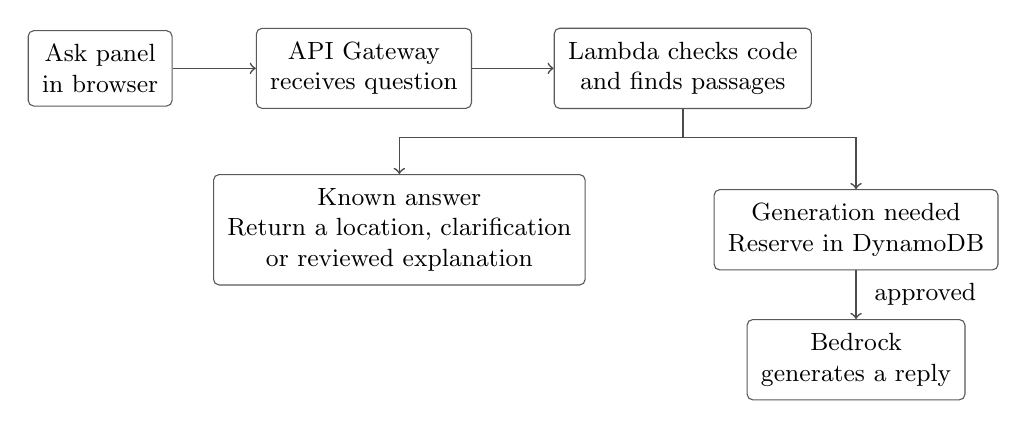
\begin{tikzpicture}[x=1cm,y=1cm,box/.style={draw=black!65,rounded corners=2pt,align=center,font=\small,inner sep=5pt},line/.style={->,semithick,draw=black!70}]
\node[box] (a) at (-4.8,0) {Ask panel\\in browser};
\node[box] (b) at (-1.45,0) {API Gateway\\receives question};
\node[box] (c) at (2.6,0) {Lambda checks code\\and finds passages};
\node[box] (d) at (-1.0,-2.05) {Known answer\\Return a location, clarification\\or reviewed explanation};
\node[box] (e) at (4.8,-2.05) {Generation needed\\Reserve in DynamoDB};
\node[box] (f) at (4.8,-3.7) {Bedrock\\generates a reply};
\draw[line] (a)--(b);\draw[line] (b)--(c);
\draw[semithick,draw=black!70] (c.south)--(2.6,-.88);
\draw[line] (2.6,-.88)-|(d.north);
\draw[line] (2.6,-.88)-|(e.north);
\draw[line] (e)--node[midway,right=3pt,font=\small]{approved}(f);
\end{tikzpicture}
\end{center}
Both paths return through Lambda and API Gateway to the same Ask panel. If the reservation fails because the monthly allowance is exhausted, the handler returns a limit message. Students can still open the notes.
\hd{Which source wins?}
\textbf{A numbered exercise.} Ask searches the open page for that number and part. The visible heading can resolve a repeated number. Several plausible matches prompt a clarification. A matching worked example elsewhere can supply a method.

\textbf{A concept question.} Passages across the book compete on word rarity, title matches and reading context. Up to two go to the model. A citation points to a published heading, so the student can check the original.

\textbf{A follow-up.} The browser supplies the current heading and up to three recent exchanges. \emph{What about (b)?} can follow a change of exercise. A check of the logarithm from the previous reply can stay with problem 12 while problem 9 is visible.

\partpage{lab}{Local lab}{A retrieval lab on your laptop}
\textbf{Question.} What information turns \emph{Help with problem 8} into an unambiguous request? Vary only the review page. This experiment runs in Python without a class code or model call.
\step{1}{Prepare a checkout}
Use Git, Python 3.11 or later, and Quarto. The publishing workflow specifies its Quarto version. In a new working directory, run the following. If you already have a checkout, start at its root, the folder containing \file{_quarto.yml}.
{\small\begin{verbatim}
git clone https://github.com/juansalinas2/Math-1334---Calculus.git
cd Math-1334---Calculus
quarto render
python3 -m unittest discover -s ask-notes -q
\end{verbatim}}
\textbf{Checkpoint.} Rendering creates \file{_site/assets/course-search-index.js}. The tests should finish with \file{OK}. If the index is missing, finish the render before running the experiment.
\step{2}{Run the same question against two pages}
Paste the following into a macOS or Linux terminal from the checkout root.
{\small\begin{verbatim}
cd ask-notes
python3 - <<'PY'
from pathlib import Path
from export import course_passages
from course_index import Index

book = course_passages(Path("../_site"))
index = Index(book)
question = "Help with problem 8"
exam2 = "lectures/exam-2-review.html"
exam3 = "lectures/exam-3-review.html"
hits, message = index.search(question, exam2, exam2)
print(book[hits[0]]["title"] if hits else message)
hits, message = index.search(question, exam3, exam3)
print(book[hits[0]]["title"] if hits else message)
PY
cd ..
\end{verbatim}}
\step{3}{Predict, then compare}
The expected lines are \emph{8. Implicit differentiation} and \emph{8. Optimization: folding a box}. Change the number to \file{99999} and rerun the block. Both reviews should ask for a heading or first line.

\textbf{What this isolates.} If these titles are right but a live reply still uses another exercise, check the browser request and the deployed index. A prompt edit would leave a stale catalog or incorrect page identifier in place.

\partpage{release}{Maintenance}{Release a change}
\textbf{Choose the file that owns the behavior.} Paths below are relative to the checkout root. One lecture correction can affect both the website and the backend's copy.
\grid{.33\linewidth}{
\textbf{Change}&\textbf{Edit here}\\\midrule
A problem, explanation or formula&Its file under \file{lectures/}. Preserve the heading identifier used by existing links.\\
What Ask treats as problem 8&\file{ask-notes/course_index.py} for matching. \file{ask-notes/practice.js} determines the visible heading.\\
How a hint or work check reads&\file{ask-notes/app.py}, beginning at \file{TEACHING}. Instructor-reviewed related-rates replies live in \file{ask-notes/checks.json}.\\}
\step{1}{Publish the website first if the notes changed}
Render and run the tests on page 3. Commit the intended edit and publish it on \file{main}. In \lnk{\repo/actions}{GitHub Actions}, wait for \emph{Publish course notes} to succeed. Open the live heading and verify the corrected formula there.
\step{2}{Refresh the backend in Oregon CloudShell}
Use the AWS account that owns the \file{math1334-ask-notes} stack in \file{us-west-2}. From a clean checkout at the release commit, run the commands below. For a first checkout, use the clone command on page 3. For an existing clean checkout on \file{main}, update it with \file{git pull --ff-only}.
{\small\begin{verbatim}
git rev-parse --short HEAD
python3 ask-notes/deploy.py --published-notes --metered \
  --verify-feedback --class-code-file ~/.math1334-class-code
\end{verbatim}}
On an existing deployment, use the original private class-code file. A missing file makes the script generate a new code, changing student access. On first setup that is intentional. AWS CLI and SAM CLI must be available. The script reads the live notes, deploys Lambda and checks a ladder citation. On a new stack, copy its printed endpoint into \file{ask-notes/pilot-endpoint.txt} and publish Pages. The feedback check submits, reads and removes synthetic examples.
\step{3}{Check the change through the student panel}
Open the revised page, start a new question, and name the edited exercise. Follow the citation to the heading and compare the answer with the edited statement. For a teaching change, try a hint and then explicitly request the calculation. Check that the second reply reaches the result.

\partpage{repair}{Troubleshooting}{Find the first wrong step}
\textbf{Record a reproducible case.} Keep the public URL, the heading shown in Ask, the exact wording, whether it was a new conversation, and the cited heading. Use an invented question when reproducing a problem in a public issue.
\grid{.31\linewidth}{
\textbf{Symptom}&\textbf{First check and repair}\\\midrule
The panel names the wrong heading.&Ask \emph{What page am I on?} after scrolling settles. Compare it with the reading. Inspect \file{currentReading()} in \file{practice.js} if the mismatch persists.\\
The heading is right but the citation is wrong.&Run the lab on page 3 using the student's page and number. If it fails locally, inspect the lecture heading and index. If it passes, compare the published heading and refresh the backend.\\
The citation is right but the teaching is wrong.&Open the cited passage. Check the givens, worked algebra and requested part. Compare a first hint with an explicit walkthrough. Inspect \file{app.py} if the source is sound.\\
The notes changed but Ask quotes the old formula.&Check the live page. If it is current, repeat the backend refresh on page 4. If it is stale, start with the Pages build.\\
A comment failed to save.&An expired or already-used receipt can produce a 409. Copy the comment, ask again for a fresh reply, then submit its form. The feedback check on page 4 verifies read-back.\\}
\hd{Read the service response}
\textbf{403} means the class-code check failed. Re-enter the current code. \textbf{429} can mean a burst of traffic or an exhausted model allowance. Read the message before retrying. \textbf{503} means the backend could not complete the request. In Oregon, open the stack's \emph{Answer} Lambda function, then \emph{Monitor} and its CloudWatch logs. Check the error category at the time of the request.
\hd{What the instructor can see}
A pending feedback receipt stores a digest and expires for sharing after two hours. Submitting an exchange through \emph{Comment or report} saves its text for instructor review with a 90-day expiry. In CloudShell, \file{python3 ask-notes/review.py} from the checkout root writes a private HTML report. A remembered class code lasts up to 90 days. The conversation stays in page memory in the browser.

\partpage{evidence}{Cost and evaluation}{Costs, evidence and tradeoffs}
\hd{What does a month cost?}
The application enforces a \textbf{\$2 monthly model allowance}. Before calling Bedrock, Lambda reserves a conservative upper bound in DynamoDB. A conditional update prevents two concurrent requests from spending the same remainder. After success, the app releases the unused reservation according to reported token usage. Ordinary replies allow 350 output tokens. An explicitly requested whole multipart solution can use 850.

\textbf{Worked estimate.} Assume 50 generated replies per week across the class, each using 2,000 input and 150 output tokens. At the rates configured in the code, a month averages
\[
  50\cdot\frac{52}{12}
  \left(\frac{2{,}000\cdot\$0.40+150\cdot\$3.00}{1{,}000{,}000}\right)
  \approx \$0.27 \quad\text{for model usage.}
\]
Use AWS Billing for actual charges. The separate \textbf{\$5 AWS Budget} tracks account spend before credits and refunds, including API Gateway, Lambda and storage. This stack has no automatic account shutdown at \$5. \lnk{https://docs.aws.amazon.com/cost-management/latest/userguide/budgets-managing-costs.html}{AWS Budgets documentation}.
\hd{What has been tested?}
From the checkout root, rerun the fixed retrieval benchmark locally.
{\small\begin{verbatim}
python3 ask-notes/benchmark/run.py score --split test \
  --output /tmp/ask-retrieval.json
\end{verbatim}}
On November 27, 2026, the system routed \textbf{31 of 35} test questions correctly. It returned an accepted passage in the first two results for 25 of 29 answerable questions and requested clarification for all six cases that required it. One miss illustrates the weakness: a question about the extra factor in differentiating \(y^2\) ranked an optimization example first. These previously examined questions now serve as regression tests.

\textbf{Assess teaching separately.} In a new dialogue, check the cited exercise, the mathematics, and whether the student received the amount of help they asked for. To assess learning itself, see whether the student can solve a similar problem independently afterward.
\hd{Explain it in an interview}
\emph{Why one index?} Exercise numbers repeat across lectures. The page tells us which set of exercises to search. An in-memory index keeps exact lookups cheap and avoids paying for an always-running search service. Its weakness is conceptual paraphrases that share little vocabulary with the notes.

\emph{What would you improve next?} Collect fresh paraphrases with instructor-labeled sources, hold out entire topics, and compare a semantic retriever with the current one on the same queries. Track correct sources, appropriate clarifications, latency and cost per question.
\end{document}
